\begin{figure}[ht]
\captionsetup[subfigure]{justification=centering}
    \centering  
    \begin{subfigure}[t]{0.5\textwidth}
        \centering   
		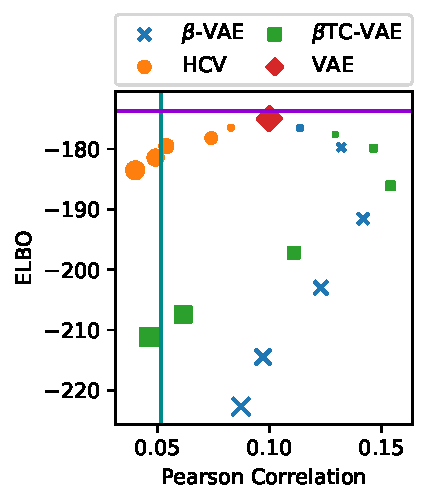
\includegraphics[width=0.7\textwidth]{figures/gaussian.pdf}
    \end{subfigure}%
    ~  
    \begin{subfigure}[t]{0.5\textwidth}
        \centering  
		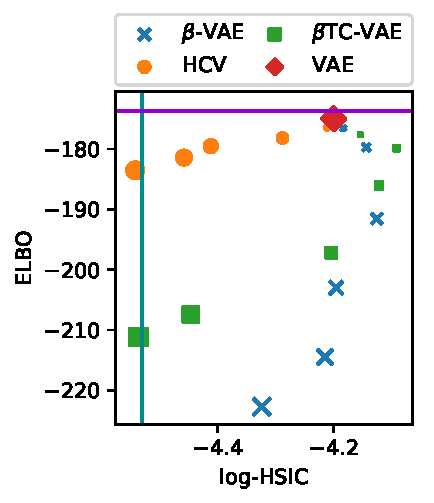
\includegraphics[width=0.7\textwidth]{figures/gaussian_hsic.pdf}
    \end{subfigure}

    \caption[Results for the linear Gaussian system]{Results for the linear Gaussian system. All results are for a test set. Each dot is averaged across five random seeds. Larger dots indicate greater regularization. The purple line is the log-likelihood under the true posterior. The cyan line is the correlation under the true posterior.}
    %\vspace{-0.5cm}
    \label{hsiclingaussfigure}
\end{figure}